\chapter{Diseño e implementación} % Main chapter title

\label{Chapter3} % Change X to a consecutive number; for referencing this chapter elsewhere, use \ref{ChapterX}

\definecolor{mygreen}{rgb}{0,0.6,0}
\definecolor{mygray}{rgb}{0.5,0.5,0.5}
\definecolor{mymauve}{rgb}{0.58,0,0.82}

%%%%%%%%%%%%%%%%%%%%%%%%%%%%%%%%%%%%%%%%%%%%%%%%%%%%%%%%%%%%%%%%%%%%%%%%%%%%%
% parámetros para configurar el formato del código en los entornos lstlisting
%%%%%%%%%%%%%%%%%%%%%%%%%%%%%%%%%%%%%%%%%%%%%%%%%%%%%%%%%%%%%%%%%%%%%%%%%%%%%
\lstset{ %
  backgroundcolor=\color{white},   % choose the background color; you must add \usepackage{color} or \usepackage{xcolor}
  basicstyle=\footnotesize,        % the size of the fonts that are used for the code
  breakatwhitespace=false,         % sets if automatic breaks should only happen at whitespace
  breaklines=true,                 % sets automatic line breaking
  captionpos=b,                    % sets the caption-position to bottom
  commentstyle=\color{mygreen},    % comment style
  deletekeywords={...},            % if you want to delete keywords from the given language
  %escapeinside={\%*}{*)},         % if you want to add LaTeX within your code
  %extendedchars=true,             % lets you use non-ASCII characters; for 8-bits encodings only, does not work with UTF-8
  %frame=single,	                 % adds a frame around the code
  keepspaces=true,                 % keeps spaces in text, useful for keeping indentation of code (possibly needs columns=flexible)
  keywordstyle=\color{blue},       % keyword style
  language=python,                % the language of the code
  %otherkeywords={*,...},          % if you want to add more keywords to the set
  numbers=left,                    % where to put the line-numbers; possible values are (none, left, right)
  numbersep=5pt,                   % how far the line-numbers are from the code
  numberstyle=\tiny\color{mygray}, % the style that is used for the line-numbers
  rulecolor=\color{black},         % if not set, the frame-color may be changed on line-breaks within not-black text (e.g. comments (green here))
  showspaces=false,                % show spaces everywhere adding particular underscores; it overrides 'showstringspaces'
  showstringspaces=false,          % underline spaces within strings only
  showtabs=false,                  % show tabs within strings adding particular underscores
  stepnumber=1,                    % the step between two line-numbers. If it's 1, each line will be numbered
  stringstyle=\color{mymauve},     % string literal style
  tabsize=2,	                     % sets default tabsize to 2 spaces
  title=\lstname,                  % show the filename of files included with \lstinputlisting; also try caption instead of title
  morecomment=[s]{/*}{*/}
}


%----------------------------------------------------------------------------------------

Este capítulo describe el diseño y la implementación de cada uno de los componentes que conforman el sistema.
Se explican las decisiones de diseño, los flujos de trabajo y los aspectos técnicos involucrados en la construcción de cada módulo principal.

%---------------------------------------------------------------------------------------
\section{Arquitectura del sistema}

El sistema está diseñado para permitir la implementación y operación de un chatbot mediante un enfoque de recuperación aumentada por generación. 
Se implementó una arquitectura modular, basada en servicios en la nube, que facilita la escalabilidad y el mantenimiento del chatbot, y permite 
una actualización ágil de los componentes y una experiencia optimizada para los usuarios finales. En la figura \ref{fig:architecture} se ilustra
el diagrama de arquitectura, donde se observan la totalidad de los componentes que conforman el sistema.

En primer lugar, los usuarios interactúan con el chatbot a través de una interfaz gráfica (desarrollada con NextUI y deployada en Azure Static Web App), 
donde consultan por la información deseada. Estas consultas son luego transferidas al servidor (Azure App Service) a través de una API desarrollada 
con la librería FastAPI. Una vez allí, se realiza un proceso de búsqueda por similitud que toma la solicitud del usuario y la compara con la información
disponible en la base de datos (Azure AI Search), con el objetivo de identificar aquellos fragmentos más relevantes. Previamente, un administrador
debe haber cargado aquellos documentos que conforman la base de conocimiento del chatbot en un repositorio de GitHub, tras lo cual se ejecuta una 
automatización que los procesa y los envía a la base de datos.

Finalmente, la consulta del usuario y los fragmentos relevantes se envían al modelo LLM (desplegado en el servicio Azure OpenAI), que genera una 
respuesta contextualizada, que es devuelta a la interfaz gráfica para ser presentada al usuario.

Además, se incluye una pequeña base de datos adicional (Azure Table Storage) que se utiliza para guardar el feedback de los usuarios, 
para así obtener métricas del desempeño del chatbot.  

\vspace{30mm}

\begin{figure}[ht]
	\centering
	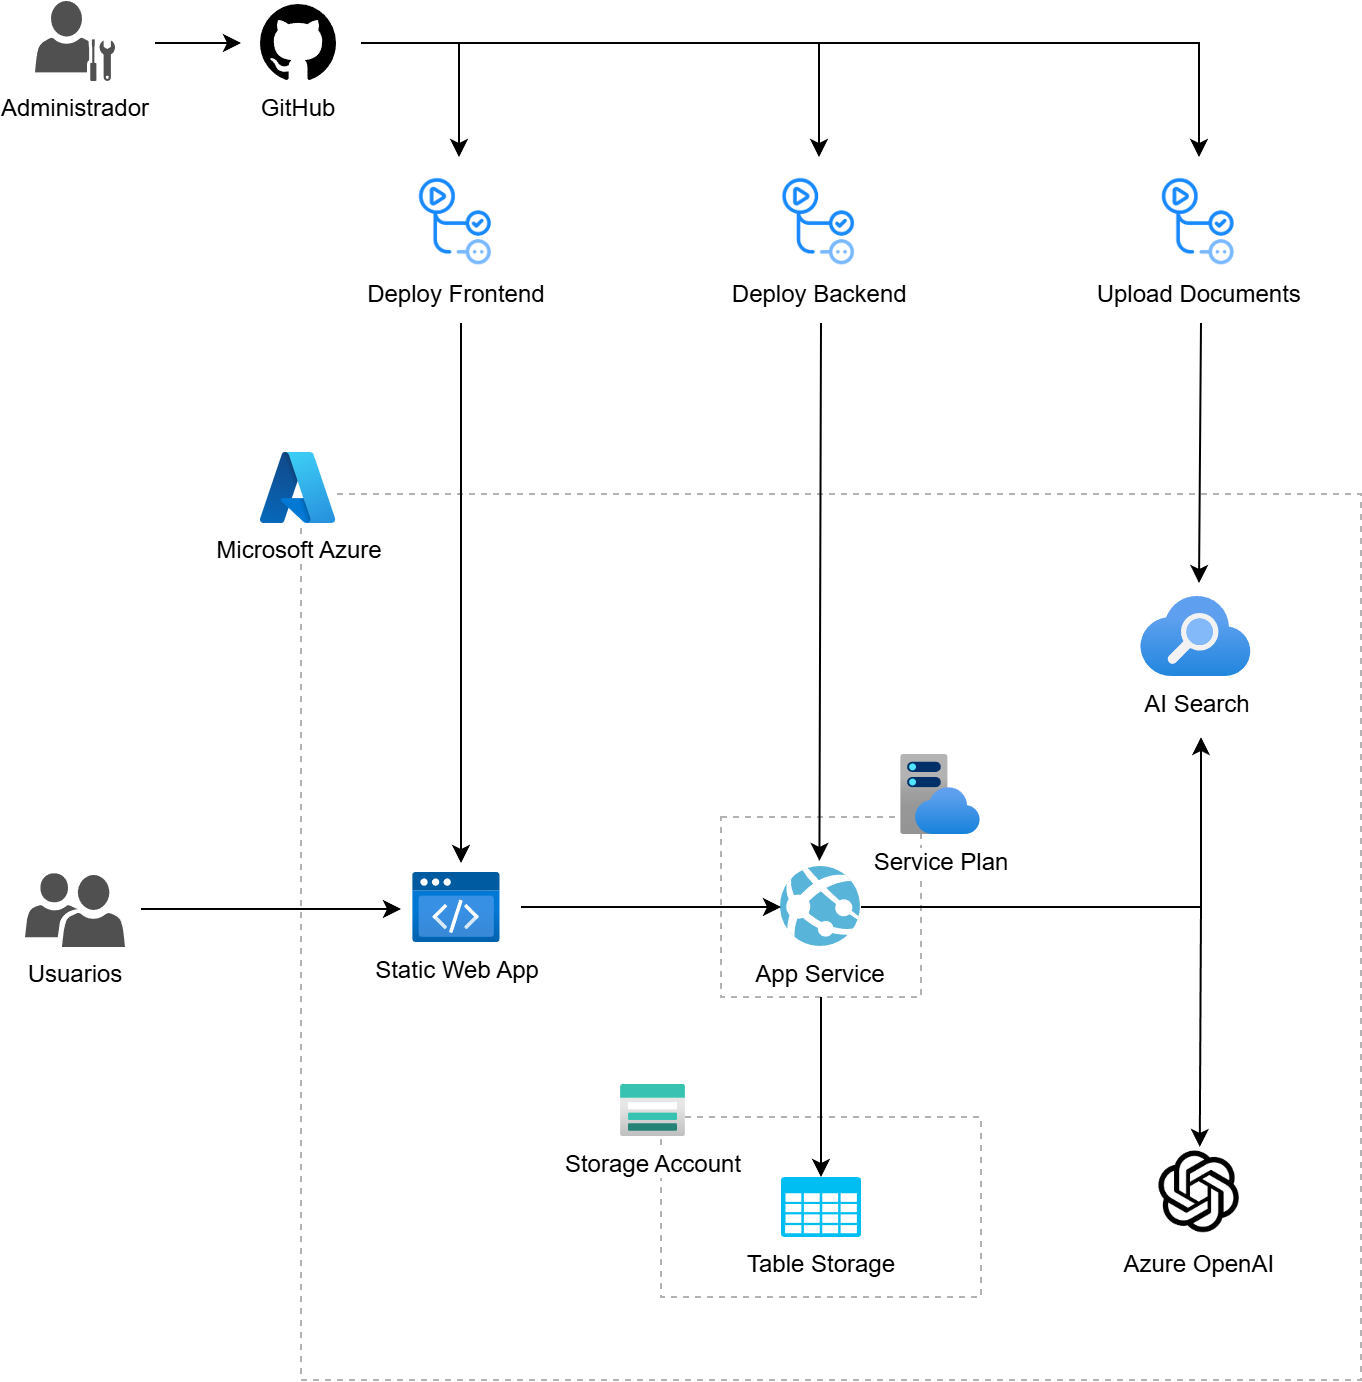
\includegraphics[scale=.55]{./Figures/arquitectura.png}
	\caption{Diagrama de arquitectura del sistema.}
	\label{fig:architecture}
\end{figure}

\vspace{8mm}

%---------------------------------------------------------------------------------------
\section{Configuración de la infraestructura en la nube}

Para garantizar el despliegue, disponibilidad y escalabilidad del sistema, se configuró una infraestructura en la nube basada en Microsoft Azure. 
A continuación, se describen los pasos principales para la configuración de cada recurso empleado en el proyecto.

\subsection{OpenAI Service}

El servicio de Azure OpenAI proporciona acceso a los potentes modelos de lenguaje de OpenAI, incluidos los más recientes. 
Estos modelos pueden adaptarse fácilmente a tareas específicas, como en este caso es la generación de contenido.

En la tabla \ref{tab:config-openai} se presenta un resumen de las configuraciones realizadas. 
Se seleccionó \textit{East US} como región, junto con el modelo de precios \textit{Standard S0}, 
adecuado para balancear el costo y el rendimiento del sistema.

Como medida de seguridad, se configuraron reglas de red para restringir el acceso únicamente al rango 
de direcciones IP del backend alojado en Azure App Service. Esto asegura que solo las solicitudes provenientes de la 
aplicación puedan acceder al modelo de lenguaje, lo que protege el servicio de accesos no autorizados.

Una vez desplegado el recurso, fue necesario seleccionar y desplegar los modelos específicos requeridos por el chatbot. 
En este caso, se optó por los siguientes modelos:

\begin{itemize}
	\item \textit{GPT-4o} como modelo de lenguaje para generación de respuestas. Este modelo está diseñado para brindar velocidad 
  y eficiencia, iguala la inteligencia de su antecesor \textit{GPT-4 Turbo}, y es notablemente más eficiente al entregar texto al 
  doble de velocidad y a la mitad del costo. Además, exhibe el rendimiento más alto en idiomas distintos del inglés en comparación 
  con los modelos de OpenAI anteriores.
	\item \textit{Ada-002} para el cálculo de \textit{embeddings} de texto. Este modelo supera a todos los modelos de \textit{embeddings} 
  anteriores en tareas de búsqueda de texto y similitud de oraciones.
\end{itemize}

Adicionalmente, es fundamental obtener el \textit{endpoint} y la \textit{key} del servicio, valores que se utilizan luego para la comunicación programática 
con Azure OpenAI. Estos datos se almacenan en el backend como variables de entorno para que el sistema pueda acceder al servicio de manera segura.

\begin{table}[h]
	\centering
	\caption[Configuración de Azure OpenAI]{Configuración de Azure OpenAI}
	\begin{tabular}{l l}    
		\toprule
		\textbf{Configuración} 	 & \textbf{Detalles} 	     \\
		\midrule
		Región                   &	East US 				 \\		
		Nivel de precios         & Standard S0				 \\
		Reglas de firewall       & Rango IP de App Service   \\
        Modelos desplegados	     & - gpt-4o				     \\
            	                 & - text-embeddings-ada-002 \\
        Credenciales	         & Endpoint y key 		     \\
		\bottomrule
		\hline
	\end{tabular}
	\label{tab:config-openai}
\end{table}

\subsection{AI Search}

Azure AI Search es un servicio de búsqueda en la nube con capacidades de inteligencia artificial integradas 
que enriquecen todo tipo de información con el fin de identificar y explorar fácilmente contenido relevante a escala.

La tabla \ref{tab:config-ai-search} presenta un resumen de las configuraciones realizadas. Se seleccionó la región de \textit{East US} y un nivel de precios 
\textit{Standard}, que ofrece hasta 50 índices para el almacenamiento y la búsqueda de documentos. En cuanto a la escala, el servicio se configuró para 
utilizar una sola unidad de búsqueda, lo cual es adecuado en principio para el volumen de consultas esperado y los requisitos de rendimiento.

Al igual que con el servicio de Azure OpenAI, se configuraron reglas de red restrictivas para mejorar la seguridad del servicio, al permitir 
únicamente el acceso desde el rango de direcciones IP asociado al backend. 

Aquí también es fundamental obtener la \textit{key} y el \textit{endpoint} del servicio para integrarlos en las variables de entorno del backend.

Es importante destacar que no es necesario crear un índice manualmente en esta etapa, ya que este será generado automáticamente como parte del pipeline de despliegue.

\begin{table}[h]
	\centering
	\caption[Configuración de Azure AI Search]{Configuración de Azure AI Search}
	\begin{tabular}{l l}    
		\toprule
		\textbf{Configuración} 	 & \textbf{Detalles} 	   \\
		\midrule
		Región                   &	East US 			   \\		
		Nivel de precios         & Standard				   \\
		Reglas de firewall       & Rango IP de App Service \\
    	Credenciales	         & Endpoint y key 		   \\
		\bottomrule
		\hline
	\end{tabular}
	\label{tab:config-ai-search}
\end{table}

\subsection{App Service}

Este servicio ofrece una plataforma completamente administrada donde es posible alojar una aplicación avanzada en la nube 
sin necesidad de manejar la infraestructura asociada. En este caso se utilizó para desplegar el backend del chatbot.

La tabla \ref{tab:config-app-service} resume la configuración principal del servicio. En primer lugar, se seleccionó un App Service Plan de categoría \textit{Basic B3}, que proporciona un poder de procesamiento de 
4 vCPU, 7 GB de memoria RAM, 10 GB de almacenamiento remoto, y permite escalar hasta 3 instancias en caso de ser necesario. 
Como entorno de ejecución, se configuró Python 3.10, mientras que como región se optó una vez más por \textit{East US}. Con el 
fin de optimizar los costos, se deshabilita la opción de redundancia zonal.

Para que la aplicación funcione correctamente, es esencial configurar un conjunto variables de entorno, que se listan en la tabla \ref{tab:config-env}. Estas 
variables incluyen las claves y los puntos de conexión de los servicios de Azure que interactúan con el backend. 

\begin{table}[h]
	\centering
	\caption[Variables de entorno en el backend]{Variables de entorno en el backend}
	\begin{tabular}{l l}    
		\toprule
		\textbf{Variable de entorno}  & \textbf{Descripción} 	                          \\
		\midrule
		openai\_api\_key              &	Clave de acceso del servicio de Azure OpenAI 	  \\		
		openai\_endpoint              & Endpoint del servicio de Azure OpenAI			  \\
		search\_key                   & Clave de acceso del servicio de Azure AI Search   \\
		search\_endpoint	          & Endpoint del servicio de Azure AI Search		  \\
        storage\_connection\_string   & Connection string de la cuenta de almacenamiento  \\
		db\_index	                  & Índice de la base de datos a utilizar		      \\
		\bottomrule
		\hline
	\end{tabular}
	\label{tab:config-env}
\end{table}

Para asegurar un monitoreo efectivo de la aplicación, se habilitó la integración con Application Insights, lo que permite un 
seguimiento detallado de las métricas de rendimiento y de uso. Adicionalmente, se configuró la opción de \textit{application logging}, 
de modo que los logs de la aplicación fueran visualizados directamente desde la terminal del App Service, facilitando la depuración 
y la supervisión continua.

\begin{table}[h]
	\centering
	\caption[Configuración de Azure App Service]{Configuración de Azure App Service}
	\begin{tabular}{l l}    
		\toprule
		\textbf{Configuración} & \textbf{Detalles} 	\\
		\midrule
		App Service Plan       & Basic B3           \\
		Runtime                & Python 3.10        \\
		Región                 & East US 			\\		
		Zone redundancy        & Deshabilitada		\\
		Application Insights   & Habilitado         \\
		Application logging	   & Filesystem			\\
		\bottomrule
		\hline
	\end{tabular}
	\label{tab:config-app-service}
\end{table}

\subsection{Static Web App}

Al utilizar este servicio, el contenido estático como HTML, CSS, JavaScript e imágenes, se distribuye globalmente desde diversos puntos 
alrededor del mundo a diferencia de un servidor web tradicional, por lo que los archivos se encuentran físicamente más cerca de los usuarios finales,
sin importar su ubicación.

La tabla \ref{tab:config-static-webapp} resume los aspectos clave de la Static Web App. Este recurso es sencillo de configurar, ya que solo requiere seleccionar un modelo de precios. En este caso, se optó por 
la versión \textit{Standard}. A diferencia de otros servicios en Azure, las Static Web Apps se despliegan globalmente, por lo que no es necesario especificar una región. 
Además, ya que todas las conexiones con otros servicios son manejadas exclusivamente por el backend, la única variable de entorno requerida 
es la URL de la API, lo que simplifica la configuración.

Es importante obtener el \textit{deployment token} asociado al recurso, que será necesario más adelante para configurar el pipeline de despliegue automático, 
permitiendo la autenticación y el despliegue seguro desde GitHub.

\begin{table}[h]
	\centering
	\caption[Configuración de Azure App Service]{Configuración de Azure App Service}
	\begin{tabular}{l l}    
		\toprule
		\textbf{Configuración} 	& \textbf{Detalles} \\
		\midrule
		Nivel de precios        & Standard          \\
		Región                  & Global 			\\		
		Variables de entorno    & URL del backend	\\
		Credenciales            & Deployment token  \\
		\bottomrule
		\hline
	\end{tabular}
	\label{tab:config-static-webapp}
\end{table}

\subsection{Table Storage}

Azure Table Storage es un servicio que almacena datos estructurados no relacionales (también conocidos como datos NoSQL) en la nube, que almacena claves/atributos 
con un diseño sin esquemas. En el contexto de este trabajo se utilizó para almacenar el feedback de los usuarios acerca de las respuestas provistas por el chatbot.

La tabla \ref{tab:config-table-storage} resume la configuración principal de este recurso. Primeramente, fue necesario desplegar una Storage Account en la región \textit{East US}, para así mantener la consistencia con los demás 
recursos del sistema. Se seleccionó una performance de tipo \textit{Standard}, adecuada para las necesidades de la aplicación.

En cuanto a la redundancia de los datos, se eligió la oferta de redundancia local, una alternativa rentable que asegura que los datos 
estén replicados dentro de un único centro de datos en la misma región, reduciendo costos sin comprometer la disponibilidad básica.

Una vez que la cuenta de almacenamiento fue desplegada, se procedió a crear la tabla que almacenará los resultados 
recopilados a través del sistema. Es importante obtener la \textit{connection string} asociada al recurso, ya que será 
necesaria para conectar la aplicación con la tabla y permitir el acceso programático. 

\begin{table}[h]
	\centering
	\caption[Configuración de Azure Table Storage]{Configuración de Azure Table Storage}
	\begin{tabular}{l l}    
		\toprule
		\textbf{Configuración} 	 & \textbf{Detalles} 	      \\
		\midrule
		Región                   &	East US 				  \\		
		Performance	             &  Standard				  \\
		Redundancia	             &  Locally-redundant storage \\
		Credenciales             &  Connection string         \\
		Nombre de la tabla       &	FeedbackTable             \\
		\bottomrule
		\hline
	\end{tabular}
	\label{tab:config-table-storage}
\end{table}

%---------------------------------------------------------------------------------------
\section{Procesamiento de los documentos}

La finalidad del procesamiento de documentos es transformar archivos de texto y PDF en un formato que facilite su búsqueda y análisis mediante 
herramientas de inteligencia artificial. Este flujo de trabajo incluye el uso de modelos de \textit{embeddings} para convertir el texto en 
representaciones vectoriales, y su posterior inserción en una base de datos vectorial. Para ello, se desarrolló un script en Python que asegura 
un manejo eficiente de grandes volúmenes de datos, al implementar mecanismos para distribuir las solicitudes a la API de Azure Search y evitar 
superar sus límites de tasa de uso, además de optimizar el almacenamiento en el índice de búsqueda.

\subsection{Importación de bibliotecas y configuración inicial}

El script comienza con la importación de las bibliotecas necesarias para realizar el procesamiento de documentos. Se utilizan paquetes específicos 
que integran funciones avanzadas para trabajar con \textit{embeddings}, carga de documentos, y búsqueda por similitud. El módulo \textit{nltk} es esencial 
para el procesamiento de texto en lenguaje natural, al proporcionar herramientas de tokenización y etiquetado de texto.

\begin{lstlisting}[label=cod:update-db-1,caption=Importación de bibliotecas y configuración inicial.]
	import os
	import requests
	from langchain_openai import AzureOpenAIEmbeddings
	from langchain_google_genai import GoogleGenerativeAIEmbeddings
	from langchain_community.vectorstores.azuresearch import AzureSearch
	from langchain_text_splitters import RecursiveCharacterTextSplitter
	from langchain_community.document_loaders import UnstructuredMarkdownLoader, PyPDFLoader
	import nltk
	import time

	nltk.download('punkt_tab')
	nltk.download('averaged_perceptron_tagger_eng')
\end{lstlisting}

\subsection{Configuración del índice de búsqueda}

Antes de insertar documentos en la base de datos, es necesario realizar una limpieza para eliminar cualquier dato previo. La función 
\textit{delete\_index} se encarga de esta tarea, enviando una solicitud de tipo \textit{DELETE} a la API de Azure Search para borrar todos 
los documentos de un índice específico.

\begin{lstlisting}[label=cod:update-db-2,caption=Configuración del índice de búsqueda.]
	def delete_index(azure_search_endpoint, azure_search_key, index_name):
		url = f"{azure_search_endpoint}/indexes('{index_name}')?api-version=2023-11-01"
		headers = {
			"Content-Type": "application/json",
			"api-key": f"{azure_search_key}"
		}
		response = requests.delete(url, headers=headers)
		if response.status_code == 204:
			print("All documents deleted successfully.")
		else:
			print(f"Failed to delete documents. Status code: {response.status_code}, Response: {response.text}")
\end{lstlisting}

Este paso es esencial para asegurar que los datos insertados sean consistentes con los documentos procesados más recientemente, evitando 
duplicación de información y permitiendo un índice limpio.

\subsection{Configuración del modelo de \textit{embeddings}}

La selección del modelo de \textit{embeddings} depende de una variable de entorno. El script soporta tanto modelos de Azure OpenAI como de Google. 
Según el modelo especificado, se inicializa una instancia de \textit{AzureOpenAIEmbeddings} o \textit{GoogleGenerativeAIEmbeddings}.

\begin{lstlisting}[label=cod:update-db-3,caption=Configuración del modelo de \textit{embeddings}.]
	if os.getenv("EMBEDDINGS_MODEL") == "openai":
		embeddings = AzureOpenAIEmbeddings(model="ada-002", openai_api_version="2024-06-01")
	elif os.getenv("EMBEDDINGS_MODEL") == "google":    
		embeddings = GoogleGenerativeAIEmbeddings(model="models/embedding-001")
	else:
		embeddings = AzureOpenAIEmbeddings(model="ada-002", openai_api_version="2024-06-01")
\end{lstlisting}

\subsection{Conexión con la base de datos}

Una vez configurado el modelo de \textit{embeddings}, el siguiente paso es instanciar una conexión con el índice de Azure Search. 
Esto permite la interacción directa con el índice y la inserción de documentos procesados.

\begin{lstlisting}[label=cod:update-db-4,caption=Conexión con la base de datos.]
	azure_search = AzureSearch(
		azure_search_endpoint=os.getenv("AZURE_SEARCH_URI"),
		azure_search_key=os.getenv("AZURE_SEARCH_KEY"),
		index_name=index_name,
		embedding_function=embeddings.embed_query
	)
\end{lstlisting}

Este objeto se utiliza posteriormente en el flujo para agregar documentos en el índice de búsqueda, una vez que hayan sido procesados y transformados en \textit{embeddings}.

\subsection{Divisor de texto}

Para manejar eficientemente documentos extensos, el script utiliza un divisor de texto para separar el contenido en fragmentos manejables 
de hasta 512 caracteres con un solapamiento de 64 caracteres entre fragmentos consecutivos. Este solapamiento asegura la continuidad del
contexto en los fragmentos resultantes.

El script busca archivos en la carpeta \textit{knowledge-base} y aplica distintos \textit{loaders} según el tipo de archivo (PDF o Markdown). Luego, 
cada archivo se divide en fragmentos utilizando el divisor de texto configurado previamente.

\begin{lstlisting}[label=cod:update-db-5,caption=Divisor de texto.]
	splitter = RecursiveCharacterTextSplitter(chunk_size=512, chunk_overlap=64)

	for root, dirs, files in os.walk('knowledge-base'):
    for file in files:
        file_path = os.path.join(root, file)
        if file.endswith('.pdf'):
            data_loader = PyPDFLoader(file_path)
        elif file.endswith('.md'):
            data_loader = UnstructuredMarkdownLoader(file_path)
        file_chunks = data_loader.load_and_split(text_splitter=splitter)
        print(f"{file_path} splitted into {len(file_chunks)} chunks")
\end{lstlisting}

\subsection{Inserción en lotes}

Para evitar alcanzar el límite de uso de la API, los fragmentos se insertan en el índice en lotes pequeños, con una demora entre cada lote. 
La función \textit{batch\_insert\_chunks} controla esta inserción en lotes, estableciendo un tamaño de lote y un tiempo de espera entre lotes.

\begin{lstlisting}[label=cod:update-db-6,caption=Inserción en lotes.]
	def batch_insert_chunks(chunks,batch_size=5,delay_between_batches=3):
    batch_count=0
    inserted_ids = []
    for i in range(0, len(chunks), batch_size):
        batch = chunks[i:i+batch_size]
        batch_count += 1
        inserted_ids_batch = azure_search.add_documents(batch)
        inserted_ids.extend(inserted_ids_batch)
        print(f"Inserted batch #{batch_count} ({len(inserted_ids_batch)} documents)")
        time.sleep(delay_between_batches)
    return inserted_ids
\end{lstlisting}

La inserción en lotes es un aspecto clave del diseño, ya que permite manejar eficientemente grandes volúmenes de datos sin interrumpir
el flujo debido a límites de solicitud.

\vspace{8mm}

%---------------------------------------------------------------------------------------
\section{Lógica de generación aumentada por recuperación}

El sistema RAG se compone de dos etapas principales:

\begin{itemize}
	\item Fase de recuperación: Se realiza una búsqueda semántica en la base de datos vectorial para identificar 
	los fragmentos más relevantes a partir de una consulta.
	\item Fase de generación: Los fragmentos recuperados se combinan con la consulta del usuario y se utilizan 
	como contexto para un modelo de lenguaje grande (LLM), que genera una respuesta contextualizada.
\end{itemize}

Este enfoque aprovecha lo mejor de ambos mundos: la precisión en la recuperación de datos específicos y 
la capacidad generativa avanzada de los LLM.

\subsection{Fase de recuperación}

La recuperación de información es una pieza clave del sistema RAG, encargada de encontrar los fragmentos más relevantes de la base de datos vectorial.

Para ello se desarrolló la clase \textit{Retriever}, cuyo código se muestra a continuación. 

\begin{lstlisting}[label=cod:retriever,caption=Clase \textit{Retriever}.]
	class Retriever():
	
		def __init__(self):
			# Embeddings model instantiation
			if os.getenv("EMBEDDINGS_MODEL") == "openai":
				self.embeddings = AzureOpenAIEmbeddings(model="ada-002", openai_api_version="2024-06-01")
			elif os.getenv("EMBEDDINGS_MODEL") == "google":    
				self.embeddings = GoogleGenerativeAIEmbeddings(model="models/embedding-001")
			else:
				self.embeddings = AzureOpenAIEmbeddings(model="ada-002", openai_api_version="2024-06-01")
	
			# Vector store instantiation
			self.vstore = AzureSearch(
				azure_search_endpoint=os.getenv("AZURE_SEARCH_URI"),
				azure_search_key=os.getenv("AZURE_SEARCH_KEY"),
				index_name=os.getenv("DB_INDEX"),
				embedding_function=self.embeddings.embed_query
			)
	
		def invoke(self, query):
			# Run a similarity search on the database for the given query
			docs = self.vstore.similarity_search(query['input'], k=3)
			print(docs)
			return self.format_docs(docs)
		
		def format_docs(self, docs):
			# Put together the results of the similarity search into one chunk of text
			return "\n\n".join(doc.page_content for doc in docs)
\end{lstlisting}

En el constructor se inicializa el modelo de \textit{embeddings} y se establece la conexión con la base de datos vectorial en Azure Search.

El método \textit{invoke} realiza una búsqueda semántica en la base de datos y devuelve los documentos más relevantes. El método utiliza la 
función \textit{similarity\_search} para recuperar los tres fragmentos más relevantes (k=3). Posteriormente, los fragmentos se 
formatean a través del método \textit{format\_docs} en un texto único que servirá como contexto para la fase de generación. Esta 
estructura garantiza que el modelo de generación reciba un contexto consolidado y relevante.

\subsection{Fase de generación}

La fase de generación utiliza los fragmentos recuperados para producir respuestas contextuales a las consultas del usuario.

Para ello se desarrolló la clase \textit{Generator}, cuyo código se muestra a continuación.

\begin{lstlisting}[label=cod:generator,caption=Clase \textit{Generator}.]
	class Generator():

		def __init__(self, retriever):
			# Instantiate a pre-trained Large Language Model from Azure OpenAI
			self.llm = AzureChatOpenAI(
				deployment_name="gpt-4o",
				api_version="2023-06-01-preview"
			)

			# The system prompt guides the model on how to respond
			self.system_prompt = (
				"You are an AI assistant for question-answering tasks."
				"You are able to answer questions related to Fabian's final project for his master degree in AI."
				"If someone asks, 'What can I ask you about?' or other similar questions, respond with the above topics."
				"If you're unsure, use the following pieces of retrieved context to answer the question." 
				"If you don't know the answer, say that you don't know."
				"If a question does not relate to Fabian's project, respond with: 'This question falls outside of my knowledge base'." 
				"Use three sentences maximum and keep the answer concise."
				"\n\n"
				"{context}"
			)

			# The prompt puts together the system prompt with the user question
			self.prompt = ChatPromptTemplate.from_messages(
				[
					("system", self.system_prompt),
					("human", "{question}"),
				]
			)

			# The parser just plucks the string content out of the LLM's output message
			self.parser = StrOutputParser()

			# The chain orchestrates the whole flow
			self.rag_chain = (
				{"context": retriever.invoke, "question": RunnablePassthrough()}
				| self.prompt
				| self.llm
				| self.parser
			)


		def invoke(self, user_question):
			# Run the chain and returns the answer generated by the LLM
			answer = self.rag_chain.invoke({"input": user_question})
			return answer
\end{lstlisting}

En el constructor se inicializan todos los componentes fundamentales: un modelo de lenguaje grande en Azure OpenAI,
el \textit{prompt} del sistema, y una cadena (\textit{rag\_chain}) que organiza el flujo completo de la consulta, 
desde la recuperación de fragmentos hasta la generación de la respuesta. Esta estructura 
garantiza que los datos recuperados se integren con la consulta del usuario antes de pasar al modelo generativo.

El \textit{prompt} establece las instrucciones que guían al modelo en la generación de respuestas, al definir 
tanto el tono como las reglas que debe seguir. Este está diseñado para:

\begin{enumerate}
	\item Concientizar al chatbot sobre su dominio de conocimiento.
    \item Incluir solo información del contexto recuperado.
    \item Evitar responder a consultas fuera del dominio del chatbot.
    \item Limitar las respuestas a tres oraciones.
\end{enumerate}

El método \textit{invoke} utiliza la cadena para procesar la consulta del usuario y generar la respuesta final.

%---------------------------------------------------------------------------------------
\section{API}

%---------------------------------------------------------------------------------------
\section{Interfaz de usuario}

%---------------------------------------------------------------------------------------
\section{Pipelines de despliegue automático}